\newpage
\section{Object Oriented Programming}

\subsection{Java Generics}
Quando dobbiamo scrivere più strutture dati che si differiscono tra loro, possiamo generalizzare usando i \textit{generics}, ovvero definendo le classi con una variabile di tipo che verrà istanziata quando creo la struttura. \\
Possiamo quindi usare i generics (più di uno) sia nella dichiarazione di classi che di interfacce.

\begin{example}
	\begin{lstlisting}
		class NewSet<T> implements Set<T> {
			List<T> theRep;
			T lastItemInserted;
		}
	\end{lstlisting}
\end{example}

Di seguito alcuni token specifi per i generics di Java:
\begin{itemize}
	\item \textbf{extends} usato dopo un generics ne definisce l'\textit{upper bound}
	\item \textbf{super} usato dopo un generics ne definisce il \textit{lowe bound}
	\item \textbf{?} indica un tipo di cui non si è a conoscenza
\end{itemize}

\noindent Se usiamo come generico un tipo che è \textbf{sottotipo} di un altro, le strutture composte da questi tipi \textbf{NON} sono l'uno sottotipo dell'altro. Si dice quindi che Java è \textbf{invariante}:
\begin{equation*}
	T2 <: T3 \centernot\implies T1<T2> \:\: <: \:\: T1<T3>
\end{equation*}
\begin{note}[Varianza per tipi]
	Sia $A(T)$ un tipo definito usando il tipo $T$:
	\begin{itemize}
		\item $A$ è \textbf{covariante} se $T<:S \implies A(T) <: A(S)$
		\item $A$ è \textbf{contravariante} se $T<:S \implies A(S) <: A(T)$
		\item $A$ è \textbf{bivariante} se è sia covariante e contravariante
		\item $A$ è \textbf{invariante} se non è covariante e conntravariante
	\end{itemize}
\end{note}
Avendo Java delle strutture modificabili e la possibilità di creare alias con tipi diversi, è necessario che sia invariante. Al contrario OCaml è \textbf{covariante} poichè non ha queste caratteristiche.
\begin{note}[Type erasure]
	Se invece di guardare alle strutture che usano i generics guardiamo gli array di tipi diversi, in quest'ultimo caso abbiamo la covarianza. Questa scelta implementativa c'è per due motivi:
	\begin{itemize}
		\item I generics sono stati implementati per permettere di controllare i tipi mentre gli array no
		\item I generics sono stati implementati in Java 5 e per garantire la compatibilità del bytecode (per evitare di riscriverlo), nella fase di compilazione viene rimossa l'informazione sui tipi, non permettendo di fare controlli a runtime. Gli array al contrario, esistendo da sempre, contengono già nativamente l'informazione del tipo e possono sollevare eccezioni a runtime.
	\end{itemize}
\end{note}
\subsection{Java Collection Framework}
Contiene classi messe a disposizione da Java per gestire le strutture dati (le collezioni):
\begin{figure}
	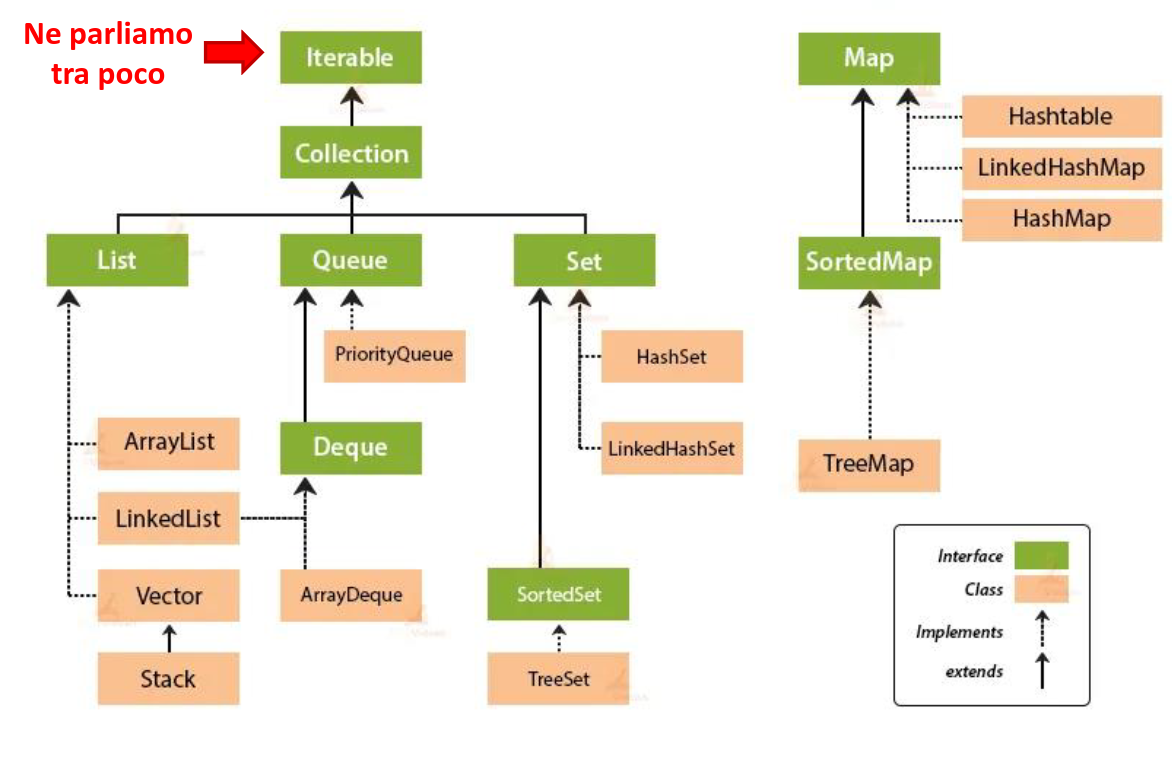
\includegraphics[width=0.98\textwidth]{jcf.png}
\end{figure}
\subsubsection{Iteratori}
Un iteratore è un'astrazione che permette di estrarre uno alla volta gli elementi di una collezione senza esporne la rappresentazione. Generalizza la scansione linerare di array e liste a collezioni generiche.
\begin{lstlisting}
	public interface Iterator<E> {
		boolean hasNext();
		E next();
		void remove();
	}
\end{lstlisting}
Quindi posso creare un iteratore su una certa collezione e poi usare quell'oggetto per scorrerla.\\
Il metodo \textbf{remove} esiste perché non si può rimuovere un oggetto dalla collezione mentre si sta visitando.\\
Tramite il \textbf{foreach} si può scorrere una collezione: Java sotto il cofano creerà un iteratore.